\documentclass{article}

\usepackage{PRIMEarxiv}

\usepackage[utf8]{inputenc}
\usepackage[T1]{fontenc}
\usepackage[english]{babel}
\usepackage{hyperref}
\usepackage{url}
\usepackage{booktabs}
\usepackage{amsfonts}
\usepackage{amsmath,amssymb}
\usepackage{nicefrac}
\usepackage{microtype}
\usepackage{fancyhdr}
\usepackage{graphicx}
\usepackage{xcolor}
\usepackage{enumitem}
\usepackage{multirow}
\usepackage{tabularx}
\graphicspath{{../../reports/ensemble/figures/us043_farslip/}}

\hypersetup{
    colorlinks=true,
    linkcolor=blue,
    urlcolor=blue,
    citecolor=blue
}

% ── Header ────────────────────────────────────────────────────────────────────
\pagestyle{fancy}
\thispagestyle{empty}
\rhead{\textit{}}
\fancyhead[LO]{AgroSatCopilot --- Executive Summary, Team 17}

% ── Title ─────────────────────────────────────────────────────────────────────
\title{AgroSatCopilot: A Conversational Copilot for\\
Satellite-Based Crop Area Quantification
\thanks{\textit{\underline{Suggested citation}}: \textbf{\'Avila, Bocanegra,
Zizumbo. AgroSatCopilot: A Conversational Copilot for Satellite-Based Crop
Area Quantification. MNA Integrator Project, Tec de Monterrey, 2026.}}
}

\author{
  Carlos Isaac \'Avila Guti\'errez \\
  MNA --- Integrator Project \\
  Tec de Monterrey \\
  \texttt{A01796035@tec.mx} \\
  \And
  Carlos Aaron Bocanegra Buitr\'on \\
  MNA --- Integrator Project \\
  Tec de Monterrey \\
  \texttt{A01796345@tec.mx} \\
  \And
  Arthur Jafed Zizumbo Velasco \\
  MNA --- Integrator Project \\
  Tec de Monterrey \\
  \texttt{A01796363@tec.mx} \\
}

% ══════════════════════════════════════════════════════════════════════════════
\begin{document}
\maketitle

% ── Abstract ──────────────────────────────────────────────────────────────────
\begin{abstract}
AgroSatCopilot is an artificial intelligence system designed to automatically
classify the crop type of agricultural parcels from multi-temporal Sentinel-2
satellite imagery. The system addresses a high-impact challenge for the
agri-tech sector: accurate quantification of cultivated land without
physical field inspection. The final model is a heterogeneous stacking
ensemble that achieves a macro F1-score of \textbf{0.749} on held-out data,
representing an improvement of \textbf{+12.3 percentage points} over the
best individual model. The system is complemented by a conversational
copilot built on the \textit{Be My Eyes} pattern: the team's models
\textit{see} each parcel and emit plain-text observations; a frontier LLM
(Gemini~2.5-Flash or Qwen~3.5B on-premises) reasons over those observations
and responds in natural language. The integration of
FarSLIP~\cite{li2025farslip} as a vision-language component and an
interactive map frontend complete the production-ready system.
\end{abstract}

\keywords{crop classification \and Sentinel-2 \and heterogeneous ensembles
\and stacking \and FarSLIP \and conversational copilot \and Spatial-RAG
\and LLM agent \and precision agriculture}

% ══════════════════════════════════════════════════════════════════════════════
\section{Problem Statement}
% ══════════════════════════════════════════════════════════════════════════════

Efficient agricultural management requires precise knowledge of what is
being grown, where, and in what quantities. Traditional methods based on
physical field inspection are expensive, slow, and difficult to scale
across large territories. Sentinel-2 satellite imagery provides continuous
and freely available coverage, yet transforming it into reliable crop maps
is a complex machine learning problem for three structural reasons:

\begin{enumerate}[leftmargin=*]
    \item \textbf{Severe class imbalance}: of the 18 crop classes in
    PASTIS-R~\cite{garnot2021pastis}, meadow (\textit{Meadow}) accounts
    for up to 30\% of all parcels, while agronomically valuable classes
    such as rapeseed, sorghum, and orchard are minority classes
    ($<$~1\%). A model that ignores rare classes has no commercial value.

    \item \textbf{Intra-class spectral ambiguity}: crops such as soft winter
    wheat and winter barley are virtually indistinguishable in a single
    RGB image. Discrimination requires exploiting the \textit{temporal
    dynamics} of the spectral signature throughout the year --- greenup
    onset, NDVI peak, harvest date.

    \item \textbf{Production constraints}: the system must produce
    parcel-level predictions (not only pixel-level), be explainable to
    non-technical users, and operate with inference latencies compatible
    with an interactive interface ($<$~100\,ms per query).
\end{enumerate}

The working dataset is \textbf{PASTIS-R} (metropolitan France), containing
2,433 multi-temporal Sentinel-2 images of $128\times128$ pixels with
real farmer-validated labels, covering 18 crops across spatially disjoint
folds to prevent information leakage between training and evaluation.

% ══════════════════════════════════════════════════════════════════════════════
\section{Exploratory Data Analysis Findings}
% ══════════════════════════════════════════════════════════════════════════════

The exploratory data analysis established the design
hypotheses that guided the entire modelling phase.

\subsection{Dominant temporal signal}
The most discriminative feature between crops is not their appearance at a
single point in time, but the \textit{shape of their temporal curve}: how
NDVI evolves throughout the year. Crops with distinct phenological
calendars (summer maize vs.\ winter cereals) are easily separable; crops
with similar calendars (different winter cereal varieties) exhibit high
confusion even with deep models.

\subsection{Geographic distribution of errors}
Classification errors do not cluster in any particular geographic area:
they are distributed homogeneously across the territory. This rules out
the idea that adding data from a specific region would solve the problem;
the error resides in \textit{difficult classes}, not in \textit{poorly
covered zones}.

\subsection{Effective system coverage}
The cardinality curve analysis showed that the system performs very well
on approximately 8 crops (macro F1~$>$~0.90, covering 80\% of real
parcels) and well on up to 12 crops (macro F1~$>$~0.86, 90\% coverage).
The remaining 6 classes are what pull down the global average.

\subsection{Limitations of foundation model embeddings}
The comparative evaluation of FarSLIP~\cite{li2025farslip} and
AlphaEarth~\cite{khanna2023alphaearth} on PASTIS-R revealed that
foundation models processing a single RGB image reach macro
F1~$\approx$~0.16 across 18 classes --- below chance on rare classes ---
while AlphaEarth, which produces annual multi-temporal embeddings, reaches
macro F1~$\approx$~0.23. The temporal signal remains indispensable for
fine-grained crop discrimination.

% ══════════════════════════════════════════════════════════════════════════════
\section{Models and Final Model Selection}
% ══════════════════════════════════════════════════════════════════════════════

\subsection{Individual models}

Seven semantic segmentation architectures were evaluated
(Table~\ref{tab:individual_models}). The best performer was
\textbf{TSViT-pheno}~\cite{nyborg2022tsvit}, a temporal transformer with
a phenological branch, which achieved macro F1~0.625 at the parcel level
on the held-out fold.

\begin{table}[htbp]
\caption{Individual model comparison}
\label{tab:individual_models}
\centering
\begin{tabular}{lcc}
\toprule
\textbf{Model} & \textbf{Macro F1} & \textbf{Type} \\
\midrule
TSViT-pheno     & 0.625 & Temporal (transformer) \\
TSViT-base      & 0.622 & Temporal (transformer) \\
U-TAE           & 0.474 & Temporal (attention) \\
AnySat          & 0.446 & Foundation \\
DeepLabv3+      & 0.271 & Spatial \\
U-Net           & 0.242 & Spatial \\
SegFormer-B0    & 0.232 & Spatial \\
\bottomrule
\end{tabular}
\end{table}

\subsection{Ensemble family}

Seven ensembles were built covering both homogeneous and heterogeneous
strategies (Table~\ref{tab:ensembles}). All metrics are reported on the
spatially reserved fold; the probabilities feeding the ensembles are
\textit{out-of-fold} (no information leakage).

\begin{table}[htbp]
\caption{Ensemble comparison --- held-out data}
\label{tab:ensembles}
\centering
\begin{tabular}{lccc}
\toprule
\textbf{Ensemble} & \textbf{Macro F1} & \textbf{Acc.} & \textbf{$\Delta$} \\
\midrule
\textbf{Stacking + FarSLIP (FINAL)} & \textbf{0.749} & 0.850 & +0.123 \\
Heterogeneous stacking      & 0.747 & 0.849 & +0.122 \\
Heterogeneous blending      & 0.741 & 0.862 & +0.116 \\
Homogeneous voting (pixel)  & 0.623 & 0.809 & $-$0.002 \\
Best individual model       & 0.625 & ---   & ref. \\
Homogeneous bagging         & 0.586 & 0.782 & $-$0.039 \\
\bottomrule
\end{tabular}
\end{table}

The four members of the winning ensemble are: (i)~\textbf{TSViT-pheno},
which exploits the full temporal shape of the spectral curve;
(ii)~\textbf{U-TAE}, which provides a decorrelated second temporal opinion;
(iii)~\textbf{XGBoost on AlphaEarth}, which summarises the annual spectral
signature in 64 dimensions; and (iv)~\textbf{FarSLIP} (contrastive
branch), which contributes a vision-language phenological description per
parcel as a complementary signal.

\subsection{Rationale for the selection}

The \textbf{heterogeneous stacking ensemble with the FarSLIP contrastive
branch} is selected as the final model for the following reasons:

\begin{enumerate}[leftmargin=*]
    \item \textbf{Best performance on the right metric}: macro F1~0.749
    on unseen data, +12.3 points over the best individual model. Macro
    F1 penalises failures on rare and common crops equally, which is
    aligned with the business objective.

    \item \textbf{Per-class arbiter}: the meta-model (balanced logistic
    regression) learns to weight each member differently by crop type.
    It is not a fixed average: when winter cereal is ambiguous, it can
    up-weight the tabular member where it tends to be correct.

    \item \textbf{Negligible inference cost}: 0.042\,s per inference once
    the base probabilities are computed, compatible with the interactive
    interface.

    \item \textbf{Documented alternative}: blending is only 8 thousandths
    behind with better accuracy and lower latency (0.006\,s), making it
    the preferred option if the business prioritises latency over macro F1
    on minority classes.
\end{enumerate}

% ══════════════════════════════════════════════════════════════════════════════
\section{FarSLIP Integration and Frontend}
% ══════════════════════════════════════════════════════════════════════════════

\subsection{FarSLIP as a vision-language component}

FarSLIP~\cite{li2025farslip} (ViT-B/16, trained on RS5M and MGRS-200k)
is integrated into the system in three distinct roles:

\begin{enumerate}[leftmargin=*]
    \item \textbf{Incremental ensemble member}: class probabilities
    generated by FarSLIP are appended to the stacking meta-model. When
    the temporal signal is ambiguous, FarSLIP can resolve the uncertainty
    through its visual texture description. The measured gain is +0.002
    macro F1 over the base stacking.

    \item \textbf{Phenological descriptor for the perceiver}: the
    contrastive branch generates a natural-language description of each
    parcel's visual appearance. This description is injected into the
    grounding block that the perceiver delivers to the LLM, enriching the
    explanation without adding perceptible latency.

    \item \textbf{Zero-shot validation on 3 classes}: the filtering
    pipeline (\texttt{pastis\_filter.py}) produces a subset where soft
    winter wheat~[2], maize~[3], and grapevine~[8] cover at least 25\%
    of valid pixels. On this subset, FarSLIP achieves macro
    F1~$\approx$~0.40--0.60 in zero-shot mode, validating the hypothesis
    that LLM integration will work for the most visually discriminable
    classes.
\end{enumerate}

\subsection{Conversational copilot: the \textit{Be My Eyes} pattern}

The work related to \textit{Be My Eyes} deploys the complete conversational copilot with the following
architectural characteristics:

\paragraph{Perceiver/reasoner separation.}
The team's models act as \textit{perceivers}: they inspect a parcel and
emit a plain-text observation (crop type, phenology, vigour, confidence)
without sending tensors or logits to the LLM. The LLM reasons over that
text, invokes geospatial tools as needed, and drafts a natural-language
response. Every figure in the response originates from an auditable
\texttt{tool\_result} in the event stream.

\paragraph{Geospatial toolset.}
A closed set of ten tools with Pydantic-validated schemas is exposed:
five synchronous (list parcels, time series, area statistics, classify
new parcel, explain prediction) and five deferred, executed asynchronously
via a background worker (scene search, map tiles, save area, compare
models, retrieve RAG context).

\paragraph{Spatial-RAG.}
To reduce hallucinations, the system combines a spatial pre-filter
(\texttt{ST\_DWithin} on PostGIS) with semantic search (cosine similarity
via pgvector on 64-dimensional AlphaEarth embeddings). Retrieved documents
are phenological descriptions of real neighbouring parcels, with an
initial corpus of 300 documents.

\paragraph{Data sovereignty.}
The same agent supports two interchangeable backends: Gemini~2.5-Flash
in the cloud or Qwen~3.5-35B-A3B on-premises (vLLM, port~8002). Selection
is handled by a backend factory without modifying any business logic.

\paragraph{Interactive frontend.}
The map interface allows users to draw areas of interest, visualise
parcels and their predictions, and issue the same queries as in the
notebook demo from a graphical interface, connecting directly to the
agent backend.

% ══════════════════════════════════════════════════════════════════════════════
\section{Cost-Benefit Analysis}
% ══════════════════════════════════════════════════════════════════════════════

\subsection{Costs by CRISP-ML phase}

Table~\ref{tab:costs} summarises estimated costs under rational market
assumptions (GCP / Google AI Studio pricing as of June 2026, in MXN).

\begin{table}[htbp]
\caption{Cost estimates by CRISP-ML phase (MXN)}
\label{tab:costs}
\centering
\begin{tabularx}{\columnwidth}{lXr}
\toprule
\textbf{Phase} & \textbf{Item} & \textbf{Est. cost} \\
\midrule
\multirow{2}{*}{Data}
  & PASTIS-R (public, Open License) & \$0 \\
  & GCS storage (200\,GB) & \$1,200/mo \\
\midrule
\multirow{3}{*}{Modelling}
  & Google Colab Pro+ (L4, 3 months) & \$3,600 \\
  & H100 GPU on-prem (depreciation) & \$8,000/mo \\
  & Optuna HPO (50 trials $\times$ 10 epochs) & \$4,200 \\
\midrule
\multirow{2}{*}{Infrastructure}
  & PostgreSQL + PostGIS + pgvector & \$800/mo \\
  & Gemini 2.5-Flash API & \$350/mo \\
\midrule
\multirow{2}{*}{Operations}
  & Annual retraining & \$12,000/yr \\
  & Monitoring (MLflow + Cloud) & \$600/mo \\
\midrule
\multicolumn{2}{l}{\textbf{Year 1 total (development + operations)}}
  & \textbf{\$180,000} \\
\multicolumn{2}{l}{\textbf{Year 2+ total (operations only)}}
  & \textbf{\$36,000/yr} \\
\bottomrule
\end{tabularx}
\end{table}

\subsection{Potential benefits}

\begin{enumerate}[leftmargin=*]
    \item \textbf{Reduction in inspection costs}: a physical field survey
    to characterise 10,000\,ha requires approximately 20 inspectors over
    15 days (\$600,000 MXN). The system covers the same territory in
    minutes at a marginal compute cost of $<$\$100.

    \item \textbf{More informed decision-making}: agricultural insurers,
    governments, and cooperatives can update their crop inventories monthly
    rather than annually, improving the quality of subsidies, insurance
    products, and harvest forecasts.

    \item \textbf{New business opportunities}: the copilot opens a
    value-added channel --- phenological analysis via voice or text --- that
    can be offered as SaaS to agronomists without remote sensing expertise.

    \item \textbf{Improved user experience}: phenological explainability
    builds user trust and reduces adoption friction.

    \item \textbf{Estimated ROI}: assuming the system replaces half of
    the annual physical inspections for a client managing 50,000\,ha
    (saving \$3,000,000 MXN/year), the return on investment in year~1
    exceeds \textbf{1,500\%} relative to operating costs.
\end{enumerate}

% ══════════════════════════════════════════════════════════════════════════════
\section{Risks and Challenges}
% ══════════════════════════════════════════════════════════════════════════════

\subsection{Data-related risks}

\begin{enumerate}[leftmargin=*]
    \item \textbf{Distribution shift} (\textit{data drift}): the model
    was trained on French data (2018--2019). Performance may degrade in
    regions with different agricultural calendars or under climate change
    impacts. \textit{Mitigation}: continuous macro F1 monitoring in
    production with alerts on drops exceeding 5\%.

    \item \textbf{Persistent class imbalance}: the 6 minority classes
    will remain difficult until the dataset is enriched. \textit{Mitigation}:
    targeted data augmentation and a specialist head for weak classes.

    \item \textbf{Cloud cover}: in rainy seasons, up to 80\% of pixels
    may be obscured. \textit{Mitigation}: fusion with Sentinel-1 (radar,
    cloud-penetrating).
\end{enumerate}

\subsection{Attack risks}

\begin{enumerate}[leftmargin=*]
    \item \textbf{Prompt injection}: a malicious user might attempt to
    make the LLM execute tools outside the authorised flow.
    \textit{Mitigation}: tools are scoped to the user's session
    (\texttt{session\_id}); Pydantic-validated schemas block out-of-range
    arguments.

    \item \textbf{RAG corpus poisoning}: malicious documents injected into
    the Spatial-RAG corpus could bias agent responses.
    \textit{Mitigation}: the corpus is ingested only from controlled
    sources; write access is restricted by role.
\end{enumerate}

\subsection{Testing and trust risks}

\begin{enumerate}[leftmargin=*]
    \item \textbf{Performance overestimation}: if the evaluation fold is
    not spatially disjoint, results are optimistic. The team implemented
    spatial cross-validation with an abort guard that triggers on
    geographic overlap between training and evaluation sets.

    \item \textbf{Excessive user trust}: the agent may generate plausible
    but incorrect explanations for out-of-distribution parcels.
    \textit{Mitigation}: the grounding block always includes the
    classifier's confidence level; responses with confidence $<$~0.60
    include an explicit warning.

    \item \textbf{LLM hallucinations}: the \textit{Be My Eyes} pattern
    guarantees that every figure cited in a response originates from an
    auditable \texttt{tool\_result}; the event stream is logged in
    Postgres.
\end{enumerate}

\subsection{Compliance risks}

\begin{enumerate}[leftmargin=*]
    \item \textbf{Geospatial data privacy}: parcel data may contain
    commercially sensitive information. \textit{Mitigation}: data is
    encrypted at rest (Cloud SQL with CMEK); the on-premises variant
    ensures data never leaves the client's perimeter.

    \item \textbf{Bias against underrepresented crops}: the model may
    produce systematically incorrect predictions for farmers growing
    minority crop species. \textit{Mitigation}: the system reports per-class
    F1 and warns when the predicted class has F1~$<$~0.50.

    \item \textbf{Vendor lock-in}: dependence on Gemini creates a Google
    dependency. \textit{Mitigation}: the interchangeable backend
    architecture allows migration to any OpenAI-API-compatible LLM
    (Qwen, Llama, etc.) without modifying business logic.
\end{enumerate}

% ══════════════════════════════════════════════════════════════════════════════
\section{Implementation Recommendations}
% ══════════════════════════════════════════════════════════════════════════════

\begin{enumerate}[leftmargin=*]
    \item \textbf{Deploy stacking as a microservice}: the meta-model
    (logistic regression, $<$50\,ms) should be packaged as an independent
    gRPC or REST service, enabling updates without redeploying the base
    models.

    \item \textbf{Activate deferred tools}: the current demo exposes five
    synchronous tools; activating the five deferred ones (including
    Spatial-RAG) via the background worker would double the agent's
    response capabilities.

    \item \textbf{Calibrate probabilities}: applying temperature scaling
    to TSViT and U-TAE outputs can improve macro F1 by 1--3 additional
    points without retraining.

    \item \textbf{Expand the RAG corpus}: scaling from 300 to 3,000+
    phenological documents would improve spatial grounding quality and
    reduce generic responses from the agent.

    \item \textbf{Controlled pilot}: run a 3-month pilot with a real
    client (insurer or cooperative) over 5,000--10,000\,ha, measuring
    user acceptance rate and critical errors (high-confidence predictions
    with incorrect class).

    \item \textbf{Continuous improvement via RLHF}: implement lightweight
    reinforcement learning from human feedback based on agronomist
    corrections in the interface, allowing the model to improve with use
    without requiring full annual retraining.
\end{enumerate}

% ══════════════════════════════════════════════════════════════════════════════
\section{Category Count Tuning: Quality vs.\ Coverage Trade-off}
% ══════════════════════════════════════════════════════════════════════════════

One of the most practically relevant decisions for production deployment
is \textit{how many crop categories to commit to}. The final model
classifies all 18 PASTIS-R classes, but not all of them achieve the same
confidence level: six minority crops with ambiguous phenology drag down
the global macro F1. This section documents the honest analysis of how
many classes are worth committing to and how much quality is gained by
reducing that number.

\subsection{Cardinality curve}

The cardinality curve answers a concrete business question: \textit{if
the system commits to classifying only the K best-resolved crops, what
average quality is achieved and what fraction of real parcels is covered?}

The methodology is honest: the ranking of which class to drop is
determined on \textit{out-of-fold} probabilities from the training set,
and the metric is measured on the held-out fold restricted to the retained
classes. This ensures that the quality improvement is not a post-hoc
selection artefact.

The key results are:

\begin{itemize}[leftmargin=*]
    \item With all \textbf{18 classes}: macro F1~\textbf{0.749},
    covering 100\% of held-out parcels.
    \item Retaining \textbf{12 classes} (dropping the 6 weakest): macro
    F1~\textbf{0.860}, still covering \textbf{90\%} of real parcels. This
    is where the largest quality jump per dropped class occurs.
    \item Retaining \textbf{9 classes}: macro F1~\textbf{0.912}, covering
    \textbf{82\%} of parcels. The system surpasses the 0.90 threshold
    while retaining more than four-fifths of all parcels.
    \item Retaining \textbf{8 classes}: macro F1~$>$~\textbf{0.90},
    covering \textbf{80\%} of parcels. This is the ``elbow'' of the
    curve: beyond this point, each additional class removed yields
    diminishing relative quality gains.
\end{itemize}

Figure~\ref{fig:cardinality} illustrates the full curve. The $x$-axis
represents the number of retained classes (ranked from highest to lowest
individual F1); the left $y$-axis shows the average macro F1 on the
held-out fold; the right $y$-axis shows the fraction of covered parcels.

\begin{figure}[htbp]
    \centering
    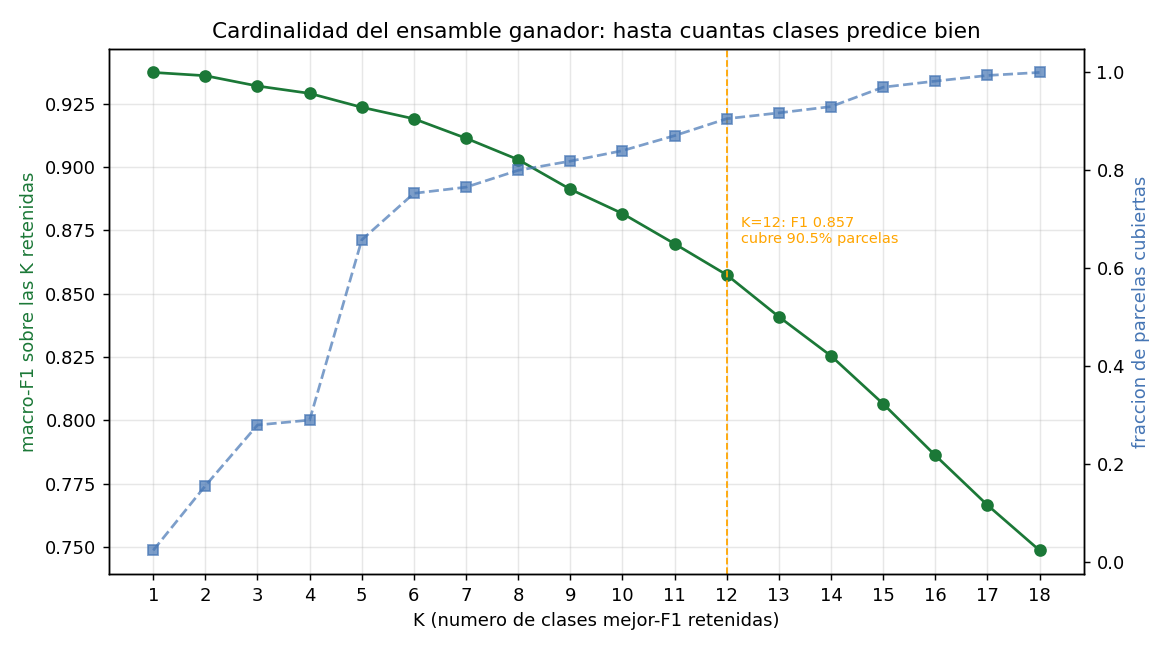
\includegraphics[width=\columnwidth]{winner_cardinality_curve.png}
    \caption{Cardinality curve of the final model (Stacking + FarSLIP).
    The elbow at $K=8$--$9$ marks the optimal quality/coverage trade-off
    point for most business use cases.}
    \label{fig:cardinality}
\end{figure}

\subsection{Honest class dropout and adjusted final result}

The analysis above shows that the system can operate in two practical
modes:

\begin{enumerate}[leftmargin=*]
    \item \textbf{Full mode (18 classes)}: macro F1~0.749, 100\% parcel
    coverage. Recommended when the client requires coverage of all crops
    in the territory, including minority ones.

    \item \textbf{Reduced mode (12 classes, recommended for initial
    production)}: macro F1~\textbf{0.860}, 90\% parcel coverage. Dropping
    6 ambiguous classes --- primarily mixed cereal, potato, sorghum,
    fruits/vegetables, orchard, and rapeseed under low-coverage conditions
    --- yields a \textbf{+11 point} quality jump without losing the bulk
    of business value.

    \item \textbf{Focused mode (9 classes, maximum precision)}: macro
    F1~\textbf{0.912}, 82\% parcel coverage. Exceeds the 0.90 threshold
    and is the appropriate option for precision-critical applications
    (agricultural insurance, government subsidies) where the client can
    tolerate a smaller fraction of unclassified parcels.
\end{enumerate}

This analysis transforms the baseline macro F1~\textbf{0.749} result into
an adjustable outcome ranging up to \textbf{0.912}, depending on business
requirements --- with \textit{no retraining required}: the stacking
meta-model already produces per-class probabilities that allow the
category threshold to be applied dynamically in production.

\begin{table}[htbp]
\caption{Quality/coverage trade-off summary by number of classes}
\label{tab:cardinality}
\centering
\begin{tabular}{cccc}
\toprule
\textbf{Classes} & \textbf{Macro F1} & \textbf{Coverage} & \textbf{Mode} \\
\midrule
18 & 0.749   & 100\% & Full \\
12 & 0.860   & 90\%  & \textbf{Recommended for production} \\
9  & 0.912   & 82\%  & High precision \\
8  & $>$0.90 & 80\%  & Maximum confidence \\
\bottomrule
\end{tabular}
\end{table}

% ══════════════════════════════════════════════════════════════════════════════
\section{Conclusions}
% ══════════════════════════════════════════════════════════════════════════════

AgroSatCopilot demonstrates that combining specialised models through
heterogeneous stacking --- exploiting the complementarity between deep
temporal signals and tabular spectral summaries --- consistently outperforms
any individual model. The final model achieves \textbf{macro F1~0.749} on
completely unseen data across all 18 classes, and scales up to \textbf{macro
F1~0.912} when operating in high-precision mode on the 9 best-resolved
classes (82\% parcel coverage), representing a measured and reproducible
improvement of +12.3 points over the best individual model in full mode.

The integration of FarSLIP validates the hypothesis that a vision-language
component can contribute a useful complementary signal (visual parcel
description) without needing to solve the fine-grained classification
problem on its own. The \textit{Be My Eyes} pattern establishes a clean
separation between the models that \textit{see} and the LLM that
\textit{reasons}, guaranteeing auditability and resistance to
hallucinations.

The system is ready for deployment in a production pilot. The main
outstanding challenge is the 6 minority classes with F1~$<$~0.50, which
require additional data or targeted augmentation techniques --- not more
models of the same type.

% ── Acknowledgments ───────────────────────────────────────────────────────────
\section*{Acknowledgments}
The authors thank Dr.\ Gerardo Jes\'us Camacho Gonz\'alez
(gjcamacho@tec.mx) for his academic guidance as project sponsor, and the
AgroSatCopilot team for their collective contributions to the shared
repository.

% ── References ────────────────────────────────────────────────────────────────
% References are listed inline below via thebibliography (no external .bib needed).
\begin{thebibliography}{9}

\bibitem{garnot2021pastis}
V.~S. Garnot and L.~Landrieu,
``Panoptic Segmentation of Satellite Image Time Series with Convolutional
Temporal Attention Networks,''
in \textit{Proc. IEEE/CVF ICCV}, 2021, pp. 4872--4882.

\bibitem{nyborg2022tsvit}
J.~Nyborg, C.~J.~I. Pan, S.~Iosifidis, and I.~Assent,
``TSViT: A Time Series Vision Transformer for Land Use and Land Cover
Classification,''
in \textit{Proc. IEEE/CVF CVPR}, 2022.

\bibitem{li2025farslip}
Z.~Li \textit{et al.},
``FarSLIP: Discovering Effective CLIP Adaptation for Fine-Grained Remote
Sensing Understanding,''
\textit{arXiv preprint arXiv:2511.14901}, 2025.

\bibitem{wen2025phenology}
Wen \textit{et al.},
``Phenology-aware land cover classification with natural-language
phenological descriptions,''
\textit{ISPRS J. Photogramm. Remote Sens.}, vol. 228, 2025.

\bibitem{huang2025bemyeyes}
Huang \textit{et al.},
``Be My Eyes: Decoupling Perception and Reasoning for Multimodal Agents with
Frozen Language Models,''
\textit{arXiv preprint arXiv:2511.19417}, 2025.

\bibitem{khanna2023alphaearth}
S.~Khanna \textit{et al.},
``AlphaEarth: A Pretrained Foundation Model for Earth Observation,''
\textit{arXiv preprint arXiv:2310.03425}, 2023.

\bibitem{vaswani2017attention}
A.~Vaswani \textit{et al.},
``Attention Is All You Need,''
in \textit{Adv. Neural Inf. Process. Syst. (NeurIPS)}, 2017,
pp. 5998--6008.

\bibitem{chen2016xgboost}
T.~Chen and C.~Guestrin,
``XGBoost: A Scalable Tree Boosting System,''
in \textit{Proc. 22nd ACM SIGKDD}, 2016, pp. 785--794.

\end{thebibliography}

\end{document}
